\chapter{Implementation} \label{chp:implementation}
This chapter will describe the implementation of the \pub{} and \sub{} as designed in the chapter \ref{chp:design}.\todo{Maybe add some more}. When referring to a requirement from the design chapter, the reference will be e.g. P1 and S1 for the \pub{} and \sub{}, respectively.

\section{Software Components}
The \pub{} and \sub{} has been implemented in PERL, as PERL is a nice language to make proof-of-concept implementations. PERL uses CPAN \footnote{\url{https://www.cpan.org/}} as package library meaning many modules are available for timeconversion, protocols etc. PERL is chosen as it is the preferred scripting language by the author and because its an exiting language to truly master.\\

\noindent{}\pro{} and \cons{} written for testing is implemented in BASH, however as described, any scripting as well as programming language could be used.\\

\noindent{} The \pro{} used for interacting with \program{Snapshot} is written in PERL as existing PERL code were available for talking to the \program{Snapshot} daemon.

\subsection{RTP/RTCP}
In order for the \pub{} and \sub{} to support sending and receiving RTP and RTCP messages a library should be used, in order not to implement parsing and composing of messages. By research, two C libraries have been found and compared. As PERL has support for wrapping C/C++ into PERL modules, one of the two modules can be integrated into the \subs{} and \pubs{}. The two libraries are oRTP and jrtplib.\\

\noindent{}\myparagraph{oRTP} 
The oRTP library is used in \textit{linphone Open-source VoIP}, which is an open-source VoIP solution created and maintained by Belledonne Communications. The oRTP library is released under the GNU GPLv2 and proprietary license meaning the library can be used for open-source projects and in proprietary solutions.
The oRTP library implements RFC3550 with an API that offers a high as well as low level interfacing for sending and receiving RTP and RTCP packets and parsing and composing RTP and RTCP packets. It supports multiple RTP sessions with IPv4 and IPv6 unicast and multicast. Furthermore, it offers support for different profiles, meaning a custom profile can be implrunmodeemented.  oRTP has a sparse documentation with only an autogenerated doxygen, where most of the functionality is described. The source-code comes with simple examples, that explains some of the library's functionality. The library is written in C and can be found in Ubuntu and Debian's packet repository. At the time of writing, the latest commit on their official github has been made 24 days ago which indicates the project is active. In CPAN, an oRTP library can be found, that implements some of the most high level API functions.


\myparagraph{jrtplib}
The jrtplib library is developed at the the Expertise Centre for Digital Media (EDM), a research institute of the Hasselt University. At the time of writing the library has been used in 61 projects listed on \href{http://research.edm.uhasselt.be/jori/cgi-bin/listprojects.py?name=jrtplib}{Project list}. The library is free to use, but must include disclaimer in the source code. The library implements RFC3550 and provides primarily a high level API, that hides most of the implementation details. The library supports parsing, composing, sending and receiving RTP and RTCP messages but does not not implement any profile, The library is written in C++ and well-documented by giving a thoroughly \textit{Getting Started} and includes 7 examples showing how to utilize the functionality of the library. Unfortunately, at the moment of writing the maintainers have not done any commits for the past year.

The libraries are compared based on the following requirements:
\begin{itemize}
	\item \textit{In repository}: From design requirement 4, the library should, if possible, be in the Debian repository.
	\item \textit{RTCP impl.}: The library should implement RTCP, as RTCP is required by the \pub{} and \sub{}.
	\item \textit{Low level API}: As the \pub{} and \sub{} should send RTCP SDEs, RTCP, BYE and RTCP SR.
	\item \textit{Custom RTP Profile}: The library should allow using a custom profile, as the \pub{} and \sub{} requires a custom profile for the non-essential/essential metadata.\todo{Verify requirement}
	\item \textit{API documented}: Preferable to ease implementation of the \pub{} and \sub{}
	\item \textit{Actively Maintained}: Relatively important, in case bugs are discovered.
	\item \textit{IPv6/4 multicast support}: Required by requirement X \todo{Analysis requirement}
	\item \textit{Existing per-binding}: As the \pub{} and \sub{} will be implemented in perl, existing bindings are preferable to ease implementation.
	\item \textit{Multiple RTP session}: Required by design requirement X
	\item \textit{Send \& Receive RTP/RTCP}: is required by \pub{} and \sub{}, respectively.
	\item \textit{Includes examples}: Preferable as it eases implementation.
\end{itemize}

\begin{table}[H]
\centering
\begin{tabular}{@{}|l|l|l@{}|}
\hline
\multicolumn{1}{|l|}{\textbf{Library property}} & \multicolumn{1}{|l|}{\textbf{oRTP}}         & \multicolumn{1}{|l|}{\textbf{jrtplib}}       \\ \midrule
\multicolumn{1}{|l|}{In repository}    & \multicolumn{1}{c|}{\checkmark} & \multicolumn{1}{l|}{} \\ \midrule
\multicolumn{1}{|l|}{RTCP impl.} & \multicolumn{1}{c|}{\checkmark} & \multicolumn{1}{c|}{\checkmark} \\ \midrule
\multicolumn{1}{|l|}{Low level API} & \multicolumn{1}{c|}{\checkmark} & \multicolumn{1}{c|}{} \\ \midrule
\multicolumn{1}{|l|}{Custom RTP Profile} & \multicolumn{1}{c|}{\checkmark} & \multicolumn{1}{c|}{} \\ \midrule
\multicolumn{1}{|l|}{API documented}          & \multicolumn{1}{c|}{\checkmark} & \multicolumn{1}{c|}{\checkmark} \\ \midrule
\multicolumn{1}{|l|}{Actively Maintained}           & \multicolumn{1}{c|}{\checkmark} & \multicolumn{1}{l|}{} \\ \midrule
\multicolumn{1}{|l|}{IPv6 multicast support}           & \multicolumn{1}{c|}{\checkmark} & \multicolumn{1}{c|}{\checkmark} \\ \midrule
\multicolumn{1}{|l|}{IPv4 multicast support}           & \multicolumn{1}{c|}{\checkmark} & \multicolumn{1}{c|}{\checkmark} \\ \midrule
\multicolumn{1}{|l|}{Existing perl-binding}           & \multicolumn{1}{c|}{\checkmark} & \multicolumn{1}{c|}{} \\ \midrule
\multicolumn{1}{|l|}{Multiple RTP sessions support}           & \multicolumn{1}{c|}{\checkmark} & \multicolumn{1}{c|}{\checkmark} \\ \midrule
\multicolumn{1}{|l|}{Send \& Receive}           & \multicolumn{1}{c|}{\checkmark} & \multicolumn{1}{c|}{\checkmark} \\ \midrule
\multicolumn{1}{|l|}{Includes examples}           & \multicolumn{1}{c|}{\checkmark} & \multicolumn{1}{c|}{\checkmark}  \\ \bottomrule
\end{tabular}
\caption{Comparesion of oRTP and jrtplib}
\label{sec:implementation:rtplib}
\end{table}

Based on the number of checkmarks in table \ref{sec:implementation:rtplib}, it has been chosen to use the oRTP library.

\todo{File tree, describe common perl library}
\subsection{Publisher \& Subscriber}

\textit{P1: The \pub{} should be the logical master of the \pro{}}\\
\textit{S1: The \sub{} should be the logical master of the \pro{}}\\

From requirement P1,S2 the \pub{} and \sub{} being the logical masters has been implemented by passing the path to the \con{} and \pro{} to the \sub{} and \pro{} respectively as an argument. This design allows the \pub{} and \sub{} to pass the pipes to the \pro{} and \con{} during run of the \con{} and \pro{}, respectively.

\begin{listing}[H] 
\begin{minted}{python}
./publisher.pl --producer producer.pl -- -v
./subscriber.pl --producer consumer.pl -- -v
\end{minted}
\caption{Example of publisher.pl run with producer.pl as parameter}
\label{code:critical_section_c}
\end{listing}

This will result in the process tree as depicted in figure \ref{sec:implementation:runmode}.

\begin{listing}[H] 
\begin{minted}{python}
/usr/bin/perl publisher.pl --producer producer.pl
 \_ /usr/bin/perl producer.pl /tmp/pub_data_pipe /tmp/pub_metadata_pipe -v
 
 /usr/bin/perl subscriber.pl --consumer consumer.pl
 \_ /usr/bin/perl consumer.pl /tmp/pub_data_pipe /tmp/pub_metadata_pipe -v
\end{minted}
\caption{Example of publisher.pl run as logical master of the producer.pl}
\label{sec:implementation:runmode}
\end{listing}

By running the consumer and producers this way gives modularity in the way the programs can be run, and does not restrict how the \con{} and \pro{} should be implemented.
Three examples shows how the \pros{}, \cons{}, \pros{} and \subs{} can be integrated with MCLURS and the streaming idea in section \ref{sec:streamingidea}.

\myparagraph{Grab with Static Metadatafile}
If \program{Grab} is used to produce data, the \con{} can be written as shown in listing \ref{lst:implementation:grab}. It should be noted that the \pro{} is a thin layer around \program{Grab}, that simply attaches \program{grab}'s stdout, to the data pipe. See section \ref{sec:implementation:ipc} for more information about the named pipes.

\begin{listing}[H] 
\begin{minted}{bash}
#!/bin/bash
# Named pipes passed as parameters
DATA_PIPE=$1
MD_PIPE=$2

# Provide feedback to the user
echo "Starting producer"

# Set non-essential metadata to Publisher
cat metadata_example.json > $MD_PIPE

# Capture samples and write to datapipe with Fs of 250kHz
/usr/bin/grab -f 2500000 > $DATA_PIPE
\end{minted}
\caption{The listing shows an implementation of a \pro{} that writes metadata and samples to the datapipe and metadatapipe, respectively}
\label{lst:implementation:grab}
\end{listing}

\noindent{}Listing \ref{lst:implementation:grab} shows how the \pro{} could be integrated with \program{grab}.
Metadata is provided by reading the \textit{metadata\_example.json}, and writing it to the metadatapipe.
As \program{grab} does not provide timing of the samples, no RTCP SR messages can be sent.


\myparagraph{Snapshot with Dynamic Metadata}
In order to use the \pub{} and \con{} with \program{Snapshot}, the \pro{} must instruct \program{Snapshot} to do repeating snapshots. Furthermore, the \program{Snapshot} must be told where it should write the samples to. This is shown as pseudocode in listing \ref{lst:implementation:snapshot1}.

\begin{listing}[H] 
\begin{minted}{python}
# Named pipes passed as parameters
DATA_PIPE=$1
MD_PIPE=$2

open MD_PIPE
write metadata.json to MD_PIPE

snapshot = ZMQ(SNAPSHOT)
snapshot.setup()
snapshot.start()
snapshot.snap(start=0,length=4096,count=100,stream=\$1)

PeriodicRun(1, updateNonessentialMetadata());


def getNonessentialMetadata():
	metadata = snapshot.getNonessentialMetaData()
	write metadata to MD_PIPE
	
\end{minted}
\caption{The listing shows an implementation of a \pro{} that writes metadata and samples to the datapipe and metadatapipe, respectively}
\label{lst:implementation:snapshot1}
\end{listing}

The setup(), start() and snap() methods implement commands used by \program{Snapshot}, in order to set parameters, start recordings and write snapshots to the pipe.
A periodic timer is created at line 16, which periodically queries the \program{Snapshot} daemon, in order to get timing information. From design requirement P10, the RTCP SR packets should be sent in order to timestamp the data stream. In order to do this, \program{Snapshot} supports ZMQ clients to query for timing information. When a \textit{Ztatus} command\footnote{Command implemented by the \program{Snapshot} daemon} is received, it sends a reply of the following format:


\begin{listing}[H] 
\begin{minted}{python}
OK Ztatus: WRITER Files 0, Xfr space 49152[ki spl]
READER ACTIVE hix: 0x0000000000824800 [spl]\ 
  tix: 000000000000000000 [spl] now: 0x00002c8008e4ee1e [ns]
\end{minted}
\caption{The listing shows an implementation of a \pro{} that writes metadata and samples to the metadatapipe and datapipe, respectively}
\label{lst:implementation:snapshot1}
\end{listing}

The important part of the reply is the \ac{HIX} and ''now``. ''Now`` is a monotonic timestamp starting at a random value, which corresponds to the \ac{HIX}. Conversion of this information into RTCP SR packets is described in section \ref{sec:design:rtcpsr}.

The converted timestamp and associated \ac{HIX} is sent via the metadatapipe as shown in line 18 to the \pro{}. In this case, the \pro{} is more than a thin layer, but it should be noted that the \pro{} never handles the data, it only parses the pipe to the \program{Snapshot}.
Figure \ref{fig:implementation:dynamicmetadata} shows how the \pub{} interacts with the \pro{} which again interacts with the \program{Snapshot} daemon.


\begin{figure}[H]
    \centering
    \begin{subfigure}[b]{0.45\textwidth}
        
\includegraphics[width=\textwidth]{figures/impl_example_snapshot_overview}
        \caption{The figure shows the communication channels between the \pub{}, \pro{} and \program{Snapshot} daemon.}
        \label{fig:implementation:dynamicmetadata}
    \end{subfigure}
    ~ %add desired spacing between images, e. g. ~, \quad, \qquad, \hfill etc. 
      %(or a blank line to force the subfigure onto a new line)
    \begin{subfigure}[b]{0.45\textwidth}
        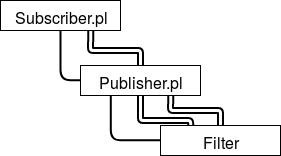
\includegraphics[width=\textwidth]{figures/impl_example_filter_overview}
        \caption{The figure shows the \textit{filter} is run by the \pub{} which is run by the \sub{}}
        \label{fig:implementation:filer}
    \end{subfigure}
\end{figure}

\myparagraph{Subscriber and Publisher with Filter}
As shown in the streaming idea section \ref{sec:streamingidea}, the system should be capable of handling a node that subscribers to a stream, and produces a new one. This will now be referred to as a filter. This can be done as showed in figure \ref{fig:implementation:filer}. In order to do do this, the \sub{} should take the \pub{} as argument, which takes the filter as argument. Unfortunately this does not work just by running the programs as described, a thin  later encapsulating the \pub{} has to be used. Listing \ref{lst:implementation:filterrun} shows how the three commands should be invoked.


\begin{listing}[H] 
\begin{minted}{bash}
perl subscriber.pl --consumer publisher.sh -- --producer filter
\end{minted}
\caption{The listing shows how a filter can be run, using the \textit{publisher.pl} and \textit{subscriber.pl}}
\label{lst:implementation:filter}
\end{listing}

If the above command is run, the process tree in listing \ref{lst:implementation:filtertree} should be seen. Due to lack of time, this has not been tested.

\begin{listing}[H] 
\begin{minted}{bash}
/usr/bin/perl subscriber.pl --consumer publisher.sh -- --producer filter
\_/bin/bash publisher.sh /tmp/datapipe1 /tmp/mdpipe1 --producer filter
  \_ /usr/bin/perl publisher.pl --producer filter -- /tmp/datapipe1 /tmp/mdpipe1
    \_./filter /tmp/datapipe2 /tmp/mdpipe2 /tmp/datapipe1 /tmp/mdpipe1
\end{minted}
\caption{The listing shows how a filter can be run, that reads data and metadata from two pipes, and writes new data and metadata to two new pipes}
\label{lst:implementation:filter}
\end{listing}
As mentioned, a bash script must be implemented, that takes the first two arguments, the datapipe and metadatapipe, and passes them to the \textit{Publisher.pl} after the $--$. If this layer is not used, the two pipes will be passed to the \textit{Publisher.pl} and not the \textit{Filter}, At the end, \textit{filter} receives four pipes, two for data and metadata input and two for data and metadata output.

\subsection{RTCP SR Timing} \label{sec:design:rtcpsr}
In order to calculate the 64 bit NTP timestamp for the RTCP SR packet, some calculations and time conversions must be done. As mentioned in the previous, the \program{Snapshot} reports a time and \ac{HIX}. This is depicted in figure \ref{fig:implementation:rtcpsr}.\footnote{This figure is a redrawing of a sketch made by John Hallam}
\begin{figure}[H]
	\centering
	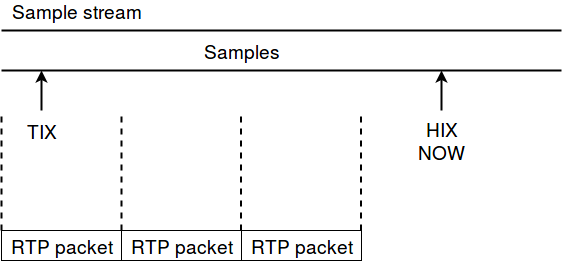
\includegraphics[width=\textwidth]{figures/rtcp_sr_timing}
	\caption{The figure shows the samples in a stream, with head(HIX) and tail(TAI) pointers. It should be noted that the ''now`` is when sample pointed to by HIX is captured}\label{fig:implementation:rtcpsr}
\end{figure}

\program{Snapchat} timestamps the sample using CLOCK\_MONOTONIC meaning the clock has a random offset but is always increasing and is thereby not affected by \ac{NTP} updates. In order to use the timestamp, this random offset has to be calculated. This calculation is shown below.

\begin{align}
	mon_1 &= parse(Ztatus).now \\
	realtime &= \text{now in UTC in seconds since epoch} \\
	mon_2 &= parse(Ztatus).now \\
	\text{UTC\_offset} &= realtime-(mon_1+mon_2)/2 
\end{align}
By getting the monotonic time before and after taking the realtime clock in UTC, the offset can be estimated by calculating the average of the monotonic time, when the realtime was captured. When the realtime clock in UTC of sample HIX should be estimated, ''now`` can simply be added to the offset.  If the calculation was done the other way around, the offset estimation would be prone to updates of NTP.

As defined in the audio/video profile, the 32 timestamp of the RTP packets should be randomly generated offsets which is incremented by the number of samples in the packet. This has been implemented by generating a random number for the offset, and adding 2048\footnote{The system has only been used with chunksize of 4096 bytes, and each sample is 2 byes} to each. When a RTCP SR packet is to be sent, the latest 32 bit timestamp has been saved saved, such that the latest RTP packet sent can be associated with the 64 bit NTP timestamp in the RTCP SR packet. In order to calculate the RTCP time of the latest sent RTP packet, the following equation has been used.
\begin{equation}
	\text{RTCP\_time} = now + Ts\cdot((latestRTP-\textit{randomRTPoffset})-HIX)+\textit{UTC\_offset}
\end{equation} \footnote{Equation formulated by John Hallam}
''now``is the timestamp at which HIX was received and Ts is the sample period.
As all timings are with respect to the linux epoch\footnote{00:00:00 UTC Thursday, 1 January 1970}, the timestamp must be converted into NTP timestamp  which pr. definitions is with respect to NTP epoch\footnote{00:00:00 UTC, January 1 1900}. After the conversion the \textit{RTCP\_time} can then be added to an RTCP SR packet together with the \textit{latestRTPtimestamp}. 
Unfortunately, this does not work. This is described in section \ref{sec:verify:rtcpsr}.

\subsection{Inter-Process Communication} \label{sec:implementation:ipc}
From implementation requirement P2/S2, the non-essential and essential metadata should be passed between the \pub{}/\sub{} and the \con{}/\pro{} using pipes. Three types of pipes are considered:
\begin{itemize}
	\item Named pipe: Named pipes or FIFO pipes in linux usually appear as files, which processes can read from and write to as part of \ac{IPC}. Named pipes are uni-directional, as one process opens the pipe for writing, and another process opens for reading. Having multiple readers from the named pipe is not supported.
	
	\item Unnamed pipe: Unamed pipes are used in linux to chain input/output between processes. As with named pipes, unamed pipes are uni-direction. This is implemented such that standard output(stdout) from one process, is attached to standard in(stdin) to the next process in the chain. As with named pipe, no framing is required.
	
	\item UNIX socket: UNIX sockets work similar to network sockets in linux, but only locally. Many clients can connect to the same server using the UNIX sockets. A UNIX socket appear like a named pipe, as a file. The UNIX socket supports bi-directional communication. 
\end{itemize}

If the \pub{} should use unnamed pipes, an unnamed pipe should be created that attach the unnamed pipe to stdout from the \pro{}, such that data printed from the \pro{} would show up at the other end of the pipe, read by the \pub{}. Another unnamed pipe could be created, that would be attached to standard error(stderr), in order to have two communication channels to pass non-essential/essential metadata and data to the \pub{}. However this design does not allow the \pro{} to generate output, which could be helpful in development, testing and debugging of \cons{}. The same could be applied to the \sub{} and \con{}; however only one communication channel is available from the \sub{} to the \con{}, which is not enough in order to provide essential/non-essential and data to the \con{}.

Unix pipes are not used, as bidirectional communication is not needed. Due to simplicity and using existing linux functionality, the communication between the \pubs{} \subs{} and \con{} and \pro{} is created using named pipes. 


\section{Publisher \& Subscriber Implementation} \label{sec:implementation:implpubsub}
From design requirements, the \pub{} and \sub{} should be implemented using events. Both prorams have been implemented using the IO::Async PERL module\footnote{\url{https://metacpan.org/pod/IO::Async}}, as it supports streaming events, meaning events from a file descriptor and periodic events.

\noindent{}PERL methods used by both the \sub{} and the \pub{} has been put into a shared library. oRTP is installed in the system, but  NET::RTP, NET::RTCP and Pubsub::Util are stored in the ''lib`` folder. The file tree is shown in listing \ref{lst:implementation:filetree}.

\begin{listing}[h] 
	\begin{minted}{bash}
|--publisher
|   |-- lib
|   |   |--- Net
|   |   |   |-- RTCP
|   |   |   |   |-- Packet.pm
|   |   |   |-- RTCP.pm
|   |   |   |-- RTP
|   |   |   |   |-- Packet.pm
|   |   |   |-- RTP.pm
|   |   |-- PubSub
|   |       |-- Util.pm
|   |-- metadata_example.json
|   |-- producer.pl -> ../producer/dummy_producer.pl
|   |-- publisher.pl
|--subscriber
|   |-- consumer.sh
|   |-- lib -> ../publisher/lib
|   |-- subscriber.pl
\end{minted}
\caption{Listing shows the tree of the files used by the \sub{} and \pub{}}
\label{lst:implementation:filetree}
\end{listing}

\subsection{Publisher}
From implementation requirement X, the following events have been implemented:
\begin{itemize}
	\item event
\end{itemize}


Listing \ref{lst:implementation:eventpublisher} shows the pseudocode of the event implementation in the \pub{}.
\begin{listing}[h] 
\begin{minted}{python}
	eventHandler = eventLoop()
	
	timerX = Timer(X, callback_Xsec)
	timerY = Timer(Y, callback_Ysec)
	
	eventHandler.add(timerX)
	eventHandler.add(timery)
	
	stream_wellknown    = getStream(fd, callback_wellknown)
	stream_source       = getStream(fd, callback_source)
	stream_sourcepipe   = getStream(source_pipe, callback_sourcepipe)
	stream_metadatapipe = getStream(metadata_pipe, callback_metadatapipe)	
	
	eventHandler.add(stream_wellknown)
	eventHandler.add(stream_source)
	eventHandler.add(stream_sourcepipe)
	eventHandler.add(stream_metadatapipe)
	
	eventHandler.run()
\end{minted}
\caption{Listing shows the event implementation in pseudocode of the \pub{}}
\label{lst:implementation:eventpublisher}
\end{listing}

From implementation requirement X, the \pub{} should take the following parameters:
\begin{itemize}
	\item P
\end{itemize}

This has been implemented, such that the \textit{Publisher.pl} can be run with the following parameters:
\begin{listing}[h] 
\begin{minted}{python}
perl publisher.pl --param1 --param2 ...
\end{minted}
\caption{Listing shows the publisher is run with the supported parameters}
\label{lst:implementation:parameterspublisher}
\end{listing}


\subsection{Subscriber}
From implementation requirement X, the following events have been implemented:
\begin{itemize}
	\item event
\end{itemize}


Listing \ref{lst:implementation:eventsubscriber} shows the pseudocode of the event implementation in the \pub{}.
\begin{listing}[h] 
\begin{minted}{python}
	eventHandler = eventLoop()
	
	timerX = Timer(X, callback_Xsec)
	timerY = Timer(Y, callback_Ysec)
	
	eventHandler.add(timerX)
	eventHandler.add(timery)
	
	stream_wellknown    = getStream(fd, callback_wellknown)
	stream_source       = getStream(fd, callback_source)
	stream_sourcepipe   = getStream(source_pipe, callback_sourcepipe)
	stream_metadatapipe = getStream(metadata_pipe, callback_metadatapipe)	
	
	eventHandler.add(stream_wellknown)
	eventHandler.add(stream_source)
	eventHandler.add(stream_sourcepipe)
	eventHandler.add(stream_metadatapipe)
	
	eventHandler.run()
\end{minted}
\caption{Listing shows the event implementation in pseudocode of the \pub{}}
\label{lst:implementation:eventsubscriber}
\end{listing}

From implementation requirement X, the \sub{} should take the following parameters:
\begin{itemize}
	\item Parameter1
\end{itemize}

This has been implemented, such that the \textit{Subscriber.pl} can be run with the following parameters:
\begin{listing}[h] 
\begin{minted}{python}
perl subscriber.pl --param1 --param2 ...
\end{minted}
\caption{Listing shows the \sub{} is run with the supported parameters}
\label{lst:implementation:parameterspublisher}
\end{listing}

From design requirement X, the \sub{} should single-handely find the multicast address from the name of a session. This has been implemented as shown as a parameter in the previous session. The parameter take a regular expression which is matched against the \textit{Session Name} of the SDP. The first SDP that matches the \textit{Session Name} will be joined.

\subsection{Composing and Parsing RTCP \& RTP Packets}
The oRTP library is used for composing RTP and RTCP packets using the NET::oRTP PERL module available from CPAN \footnote{\url{https://metacpan.org/pod/Net::oRTP}}. However the NET::oRTP module did not provide lowlevel API functions needed by the \pub{} and \sub{} to send the RTCP SDR/SR/BYE packets manually. The highlevel API could not be integrated with the IO::Async, as the oRTP library runs its own scheduler to send and receive RTP/RTCP packets. Therefore, new methods where added to the NET::oRTP library. These methods are listed below:

\begin{itemize}
	\item raw\_rtcp\_bye\_send(session, reason): Used to send the RTCP BYE packet when the \pub{} or \sub{} is shutting down gracefully.
	\item raw\_rtcp\_sdes\_send(session): Sends the RTCP SDES packet. The items are filled in using set\_sdes\_items.
	\item set\_sdes\_items(session, cname): Used to set the \ac{CNAME} in the SDES packet.
	\item raw\_rtcp\_sr\_send(session, ntpTimestamp): used to send the 64 bit timestamp. The oRTP library keeps track of the RTP timestamp of the last send RTP message.
	\item raw\_rtp\_send(session, payload): used to send an RTP packet.
\end{itemize}
The ''sesson`` is passed by PERL, when the methods are run on an object representing an RTP session. In order to use the IO::Async eventloop to handle incoming RTP and RTCP packets, the parser implemented in the oRTP library was not used due to oRTP lib's own scheduler. All RTP/RTCP sockets are created by oRTP lib, but the file descriptors are passed from the oRTP library to IO::Async's list of file descriptors to wait for.  NET::RTP\footnote{\url{https://metacpan.org/pod/Net::RTP}} and NET::RTCP \footnote{\url{https://github.com/njh/perl-net-rtp} - Written by the same guy as NET::RTP} were used to parse the received packets with success.\\

\noindent{}From design requirement X, the multicast traffic should also work on a virtual interface. In order for this to work, the IPV6\_MULTICAST\_LOOP\footnote{\url{https://docs.oracle.com/cd/E19683-01/806-4125/sockets-13/index.html}} option of the socket must be set to 1. This is supported by the set\_multicast \_loopback(session, enable) method available in the NET::oRTP library.

\section{Metadata}
Metadata must be provided by the \pro{}, as the \pro{} should be implemented to collect essential and non-essential metadata.



\todo{Describe essential and non-essential metadata}
\section{Historian}
As described in section \ref{sec:design:historian}, \program{tcpdump/tcpreplay} is used as \hist{}.
In order to record RTP and RTCP packets, \program{tcpdump} is shown in listing \ref{cmd:implementation:tcpdump}.
\begin{listing}[h] 
\begin{minted}{bash}
tcpdump -i interface -w /tmp/filedump.pcap dst port 5004 or dst port 5005 
\end{minted}
\caption{Listing shows how tcpdump is run to record RTP and RTCP packets. Port 5004 and 5005 is used for RTP and RTCP respectively}
\label{cmd:implementation:tcpdump}
\end{listing}


For replaying a recording, \program{tcpreplay} is used as showed in listing \ref{cmd:implementation:tcpreplay}. --enet-smac is used to change the MAC-address of all the packets such that they come from the right MAC-address of the physical machine replaying the packets.
\begin{listing}[h] 
	\begin{minted}{bash}
tcpreplay-edit -i eth0 --enet-smac <MAC of eth0> file1.pcap file2.pcap ...
	\end{minted}
\caption{Listing shows how tcpdump is run to record RTP and RTCP packets. Port 5004 and 5005 is used for RTP and RTCP respectively}
\label{cmd:implementation:tcpreplay}
\end{listing}

\section{Metadata profile} \label{sec:implemented:metadataprofile} 
A profile must be defined, in order to define a new set of parameters for the RTP packet such that RTP packets can carry SDP files and  non-essential metadata. At the moment of writing, the metadata profile inherent all properties from the audio/video profile, however the semantics of the  \textit{Marker}-bit has changed.

\begin{itemize}
	\item \textbf{Marker bit}: The \textit{Marker}-bit is used to denote whether the RTP packet announces a new frame or provides metadata.
		\begin{itemize}
			\item 0, the RTP packet announces a stream. 
			\item 1, the RTP packet contains non-essential metadata.
		\end{itemize}
\end{itemize}

More details should be added if RTP fields are used for other purpose than the Audio/Video profile defines.

\section{Multicast IP} \label{sec:implementation:multicastip}
Multicast for IPv4 and IPv6 does not work for all ranges of IPs, but only for a certain range allocated for multicast traffic.\footnote{\url{https://en.wikipedia.org/wiki/Multicast\_address}} 
A subset of this range is assigned to be used on a local network. 
A thorough description of the IP addresses are out of the scope of this thesis. 
For the SAP protocol\citep{RFC2974} the highest IP in the IPv4 Administrative Scope is used for announcements: 239.0.0.0 to 239.255.255.255. For the data multicast group, the 224.0.0.0 to 224.0.0.255 range can be used.

\noindent{}For IPv6 SAP uses FFYX:0:0:0:0:0:2:7FFE for session announcements. The scope of the IPv6, the X, should be set to the same scope as the actual data multicast groups such that when a participant receives a session announcement, it can join the data multicast group. The Y should be set to zero, as this means the session announcement is broadcasted. If Y is set to 1, only hosts that has joined that particular group receives the session announcement. FF is assigned to multicast addresses. For data multicast groups, any IP starting with FF1X:: can be used, where X is the scope.

\noindent{}Throughout the test verification section, FF15::beef has been used for announcements and FF15::random has ben used for data multicast groups.


%\section{Software Components}
%The following examples are made in order to show the modularity of the system:

%\section{Test}
%From wireshark after resample:
%4096 = payload
%8 bytes = data gram
%12 bytes rtp header
%
%4116 bytes i total





%\section{Verification} \label{sec:design:verification}
Several of the implementation requirements have been addressed in the chapter \ref{sec:implementation}. In order to verify the implementation and there by design works, 7 tests have been conducted.
\todo{Add what has not been fully implemented}

\todo{Describe in list which requirements are tested.}
\begin{itemize}
	\item \textbf{Session Announcement (Essential metadata)}\\
This test aims to verify the Session Announcement Mechanism with Essential metadata works as intended.
	\item \textbf{Presence Mechanism}\\
This test aims to verify the Presence Mechanism works as intended.
	\item IP collision resolver
This test aims to verify the \pub{} is able to generate a new multicast IP if there is a collision.
	\item Subscribe resolve MG
This test verifies the \sub{} can tage a session name, and resolve that into an multicast IP.
	\item Non-essential Metadata
This test verifies non-essential metadata can be sent and received.
	\item Record with tcpdump and replay with tcpreplay and see subscriber get same data.
This test verifies a stream can be recorded and replayed.
	\item Verify RTCP SR timestamps
This test is supposed to verify RTP SR timestamps are working, however at the moment of writing it does not work.
	\item Compare output from \con{} with output from \program{Snapshot}.
This verifies data sent from snapshot is the same as the \con{} receives.
\end{itemize}


\subsection{Session Announcement \& Essential metadata} \label{sec:verify:sessionannouncement}
This test verifies implementation requirement P8,P9 and S3. The goal of the test is to verify a SDP sent by a \pub{}, and verify a \sub{} can join an announced stream. \todo{add essential metdata tot}
The test has been conducted by staring a \pub{} that streams data from a \con{} which interfaces \program{Snapshot}. In order to verify the SDP is sent as an RTP packet, the traffic sent by the \pub{} has been inspected by \program{tcpdump}. Listing \ref{cmd:verify:sdp} shows the SDP packet sent by the \pub{}.

\begin{listing}[H] 
\begin{minted}{bash}
v=0
o=suas 3736400647 3736400647 IN IP4 batbox3
s=My Session
i=A fun session
u=http://www.ecs.soton.ac.uk/fun/
t=3736400647 3736404247
a=tool:publisher.pl uuid: E9A60146-618C
m=audio 5004 RTP/AVP 96
c=IN IP6 ff15::1234/5
a=quality:5
a=rtpmap:96 L16/220500/1
\end{minted}
\caption{SDP printed by the \pub{}}
\label{lst:verify:sdp}
\end{listing}

Figure \ref{lst:verify:tcpdumpsdp} shows the output from \program{tcpdump}.

\begin{listing}[H] 
	\begin{minted}{bash}
sudo tcpdump -i eth0 -X port 5004
11:04:08.895637 IP6 batbox3.local.5004 > ff15::beef.5004: UDP, length 270
        0x0000:  6006 4601 0116 110a fe80 0000 0000 0000  `.F.............
        0x0010:  ba27 ebff fe5e 2624 ff15 0000 0000 0000  .'...^&\$........
        0x0020:  0000 0000 0000 beef 138c 138c 0116 e83d  ...............=
        0x0030:  8000 0000 0001 e240 23e2 c753 763d 300a  .......@#..Sv=0.
        0x0040:  6f3d 7375 6173 2033 3733 3634 3030 3634  o=suas.373640064
        0x0050:  3720 3337 3336 3430 3036 3437 2049 4e20  7.3736400647.IN.
        0x0060:  4950 3420 6261 7462 6f78 330a 733d 4d79  IP4.batbox3.s=My
        0x0070:  2053 6573 7369 6f6e 0a69 3d41 2066 756e  .Session.i=A.fun
        0x0080:  2073 6573 7369 6f6e 0a75 3d68 7474 703a  .session.u=http:
        0x0090:  2f2f 7777 772e 6563 732e 736f 746f 6e2e  //www.ecs.soton.
        0x00a0:  6163 2e75 6b2f 6675 6e2f 0a74 3d33 3733  ac.uk/fun/.t=373
        0x00b0:  3634 3030 3634 3720 3337 3336 3430 3432  6400647.37364042
        0x00c0:  3437 0a61 3d74 6f6f 6c3a 7075 626c 6973  47.a=tool:publis
        0x00d0:  6865 722e 706c 2075 7569 643a 2045 3941  her.pl.uuid:.E9A
        0x00e0:  3630 3134 362d 3631 3843 0a6d 3d61 7564  60146-618C.m=aud
        0x00f0:  696f 2035 3030 3420 5254 502f 4156 5020  io.5004.RTP/AVP.
        0x0100:  3936 0a63 3d49 4e20 4950 3620 6666 3135  96.c=IN.IP6.ff15
        0x0110:  3a3a 3132 3334 2f35 0a61 3d71 7561 6c69  ::1234/5.a=quali
        0x0120:  7479 3a35 0a61 3d72 7470 6d61 703a 3936  ty:5.a=rtpmap:96
        0x0130:  204c 3136 2f32 3230 3530 302f 310a       .L16/220500/1.
	\end{minted}
\caption{The listing shows the output from \program{tcpdump}, listening on the well known multicast group. The bytes shown before the SDP packet is the ethernet header, UDP header and RTP header}
\label{lst:verify:tcpdumpsdp}
\end{listing}

It should be noted that the ASCII encoded content of the payload corresponds to the SDP packet in listing \ref{lst:verify:sdp}. Furthermore, a session is announce in the key starting with \textbf{C=IN...}.

In listing \ref{lst:verify:subsdp} is the output from a \sub{} shown, that receives the SDP.


\begin{listing}[h] 
\begin{minted}{bash}
SDP from 'publisher.pl uuid: E9A60146-618C', format: audio/L16/220500/1,\
	Multicast: ff15::1234:5004
Joining multicast group: ff15::1234:5004
<SDP printet>
Main-loop stopped with retval: NewRtp
Restarting loop due to new RTP stream joined
\end{minted}
\caption{Listing shows the output from a \sub{} that receives the SDP and joins the stream. It should be noted the event-loop is restarted, in order to also listen for the new multicast group}
\label{lst:verify:subsdp}
\end{listing}



\subsection{Presence Mechanism} \label{sec:verify:presencemechanism}
This test verifies implementation requirement P11-13 and S3. The goal of this test is to verify the presence mechanism works in both \sub{} and \pub{}. Due to lack of time, lists maintaining present participants have not been implemented, however RTCP SDES/BYE are sent and received by both \pub{} and \sub{}.
A test was conducted, where the \pub{} is started and some time later the \sub{} is started. The RTCP SDES sent by the \pub{} and \sub{} is shown in figure \ref{fig:verify:wireshark_presence}.

\begin{figure}[H]
	\centering
	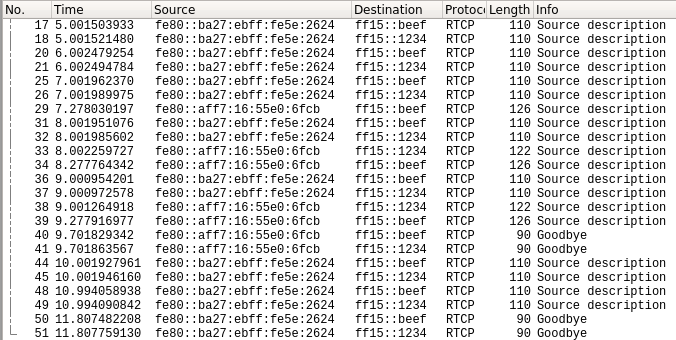
\includegraphics[width=\textwidth]{figures/wireshark_presence}
	\caption{Figure shows output from \program{Wireshark}. It should be noted, that until packet nr.26 is only fe80::ba27:.. sending RTCP SDES, but when \sub{} joins, it starts sending RTCP SDES to both the well known address ff15::beef and the source multicast group ff15::1234.} \label{fig:verify:wireshark_presence}
\end{figure}
From figure \ref{fig:verify:wireshark_presence} the RTCP SDES packets can be seen. Until packet no. 26 is only the \pub{} running. It can be seen that the \pub{} sends its RTCP SDES to both the well known multicast address(ff15::beef) and its source stream (ff15::1234). From packet nr.29, the \sub{} has been started, where it sends out an RTCP SDES to the well known multicast group. It has then joind the source multicast announced by the \pub{} from message no. 32, as the \sub{} sends RTCP SDES to the source stream too. From message no. 40 is the \sub{} gracefully shutting down as it sends a RTCP BYE to both source and well known multicast group. From message no. 50, the \pub{} is gracefully shutting down too.

Listing \ref{lst:verify:rtcpsdes} shows the ouput from a \sub{} receiving and parsing an RTCP SDES packet.

\begin{listing}[h] 
\begin{minted}{bash}
\$VAR1 = bless( {
                 'sdes' => {
                             '6c73c635' => {
                                             'LOC' => '',
                                             'PHONE' => '',
                                             'NAME' => '',
                                             'TOOL' => 'MCLURS',
                                             'NOTE' => '',
                                             'CNAME' => 'suas@batbox3',
                                             'EMAIL' => ''
                                           }
                           }
               }, 'Net::RTCP::Packet' );
\end{minted}
\caption{Listing shows part of the output from a \sub{} receiving and parsing an RTCP SDES packet sent by a \pub{}}
\label{lst:verify:rtcpsdes}
\end{listing}


\subsection{}

\begin{itemize}
	\item Tested with Lua/(post dissector) in wireshark. Transfer chunk of data of 4096 kb(page size) with counter in start of packet. Packet is read from wireshark and by writing dummy producer of 'X' x 4096.

	\item Show Byes are sent when publisher/subscriber are shutdown gracefully

	\item Show essential metadata are sent periodically as json/yml
	\item Show SDES \& BYE to both RTP sessions
	
\end{itemize}


